% =====================================================================
%  Discussão — OpenAlex: IA nas Humanidades em perspectiva internacional
%  Trecho pronto para inserir na tese. Requer \usepackage{graphicx}.
%  As figuras são geradas por figuras_openalex.py (pasta figuras/).
%  Números: ver docs/decisoes_metodologicas.md, bloco IV (fonte canônica).
% =====================================================================

\subsection{A produção de IA nas Humanidades em perspectiva internacional (OpenAlex)}

Para situar o caso brasileiro num horizonte global, recorremos a uma terceira
fonte, o \textit{OpenAlex} --- catálogo aberto de cerca de 250 milhões de obras
acadêmicas. Diferentemente da CAPES e do SciELO, restritos ao Brasil,
o OpenAlex permite comparar países e disciplinas. Adotamos como recorte de
``Humanidades'' a união dos \textit{fields} \textit{Arts and Humanities},
\textit{Psychology} e \textit{Social Sciences} (na taxonomia do OpenAlex,
herdada da Scopus/ASJC), de modo a espelhar a grande área ``Ciências Humanas''
da CAPES, que igualmente abriga a Psicologia. A janela analisada é
2016--2024, e a identificação de obras de IA combina o conceito
\textit{Artificial intelligence} do OpenAlex com a mesma régua de palavras-chave
empregada nas demais fontes (\texttt{utils.classificar\_subcampos}).

É preciso, de saída, distinguir duas definições de ``IA'' que produzem
magnitudes distintas sobre a \emph{mesma} base. Pela tag conceitual do OpenAlex,
o Brasil registra 9.996 obras de IA nas Humanidades no período; pela régua de
palavra-chave --- a mesma que sustenta os números da CAPES e do
SciELO ---, apenas 849 obras únicas mencionam, de fato, vocabulário de IA em
título ou resumo. Ou seja, somente cerca de 8,5\% das obras que o classificador
do OpenAlex sinaliza como ``IA'' contêm esse vocabulário explícito --- diferença
atribuível tanto à generosidade do conceito algorítmico quanto à ausência de
resumo em parte das obras. As comparações internacionais de volume e penetração
(Figuras~\ref{fig:openalex-ranking}, \ref{fig:openalex-taxa}
e~\ref{fig:openalex-brasil-temporal}) empregam a definição por conceito, mais
inclusiva e uniforme entre países; a análise de subcampos
(Figura~\ref{fig:openalex-subcampos}) emprega a régua de palavra-chave,
comparável às outras fontes.

% ---------------------------------------------------------------------
\begin{figure}[htbp]
  \centering
  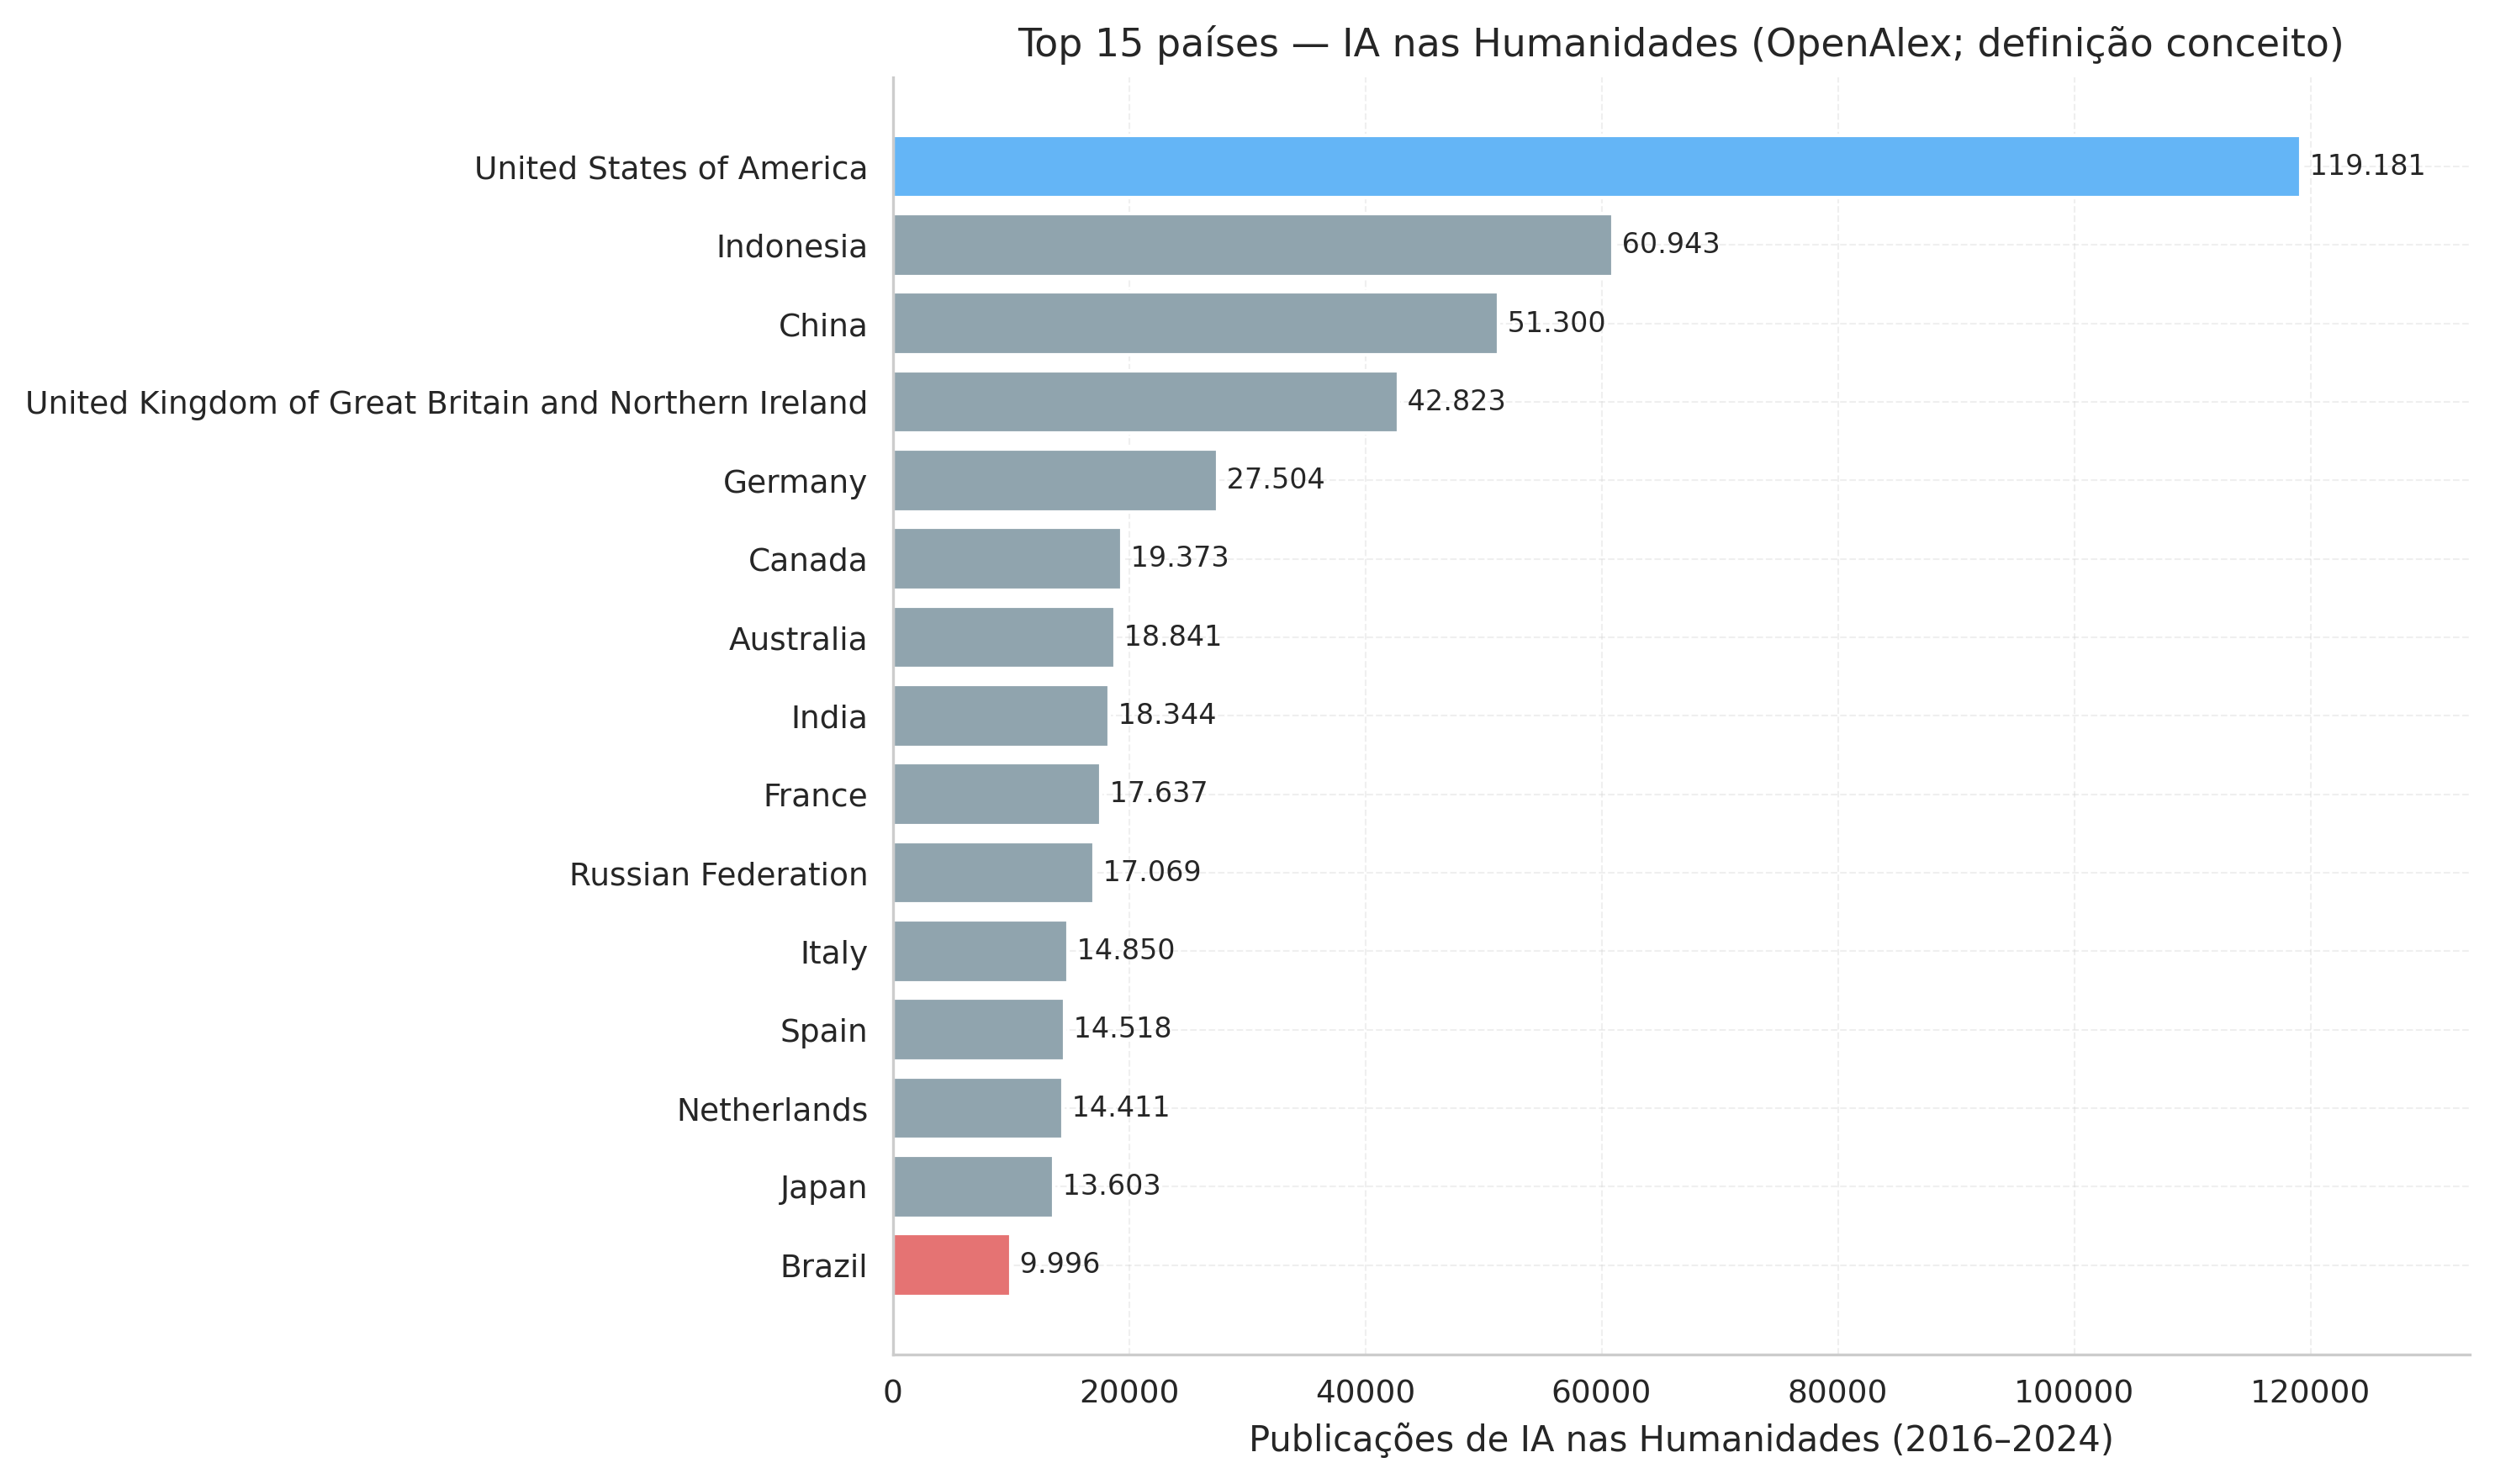
\includegraphics[width=0.95\linewidth]{figuras/openalex_01_ranking_paises.png}
  \caption[Ranking de países por volume de IA nas Humanidades (OpenAlex,
  2016--2024)]{Os quinze maiores produtores de publicações sobre inteligência
  artificial na grande área de Humanidades, 2016--2024, segundo o OpenAlex
  (definição por conceito). O Brasil, destacado, ocupa a 14.\textsuperscript{a}
  posição mundial. Fonte: elaboração própria a partir do OpenAlex.}
  \label{fig:openalex-ranking}
\end{figure}

A Figura~\ref{fig:openalex-ranking} evidencia forte concentração geográfica: os
Estados Unidos (cerca de 60,9 mil obras) e a China (51,3 mil) lideram com larga
vantagem, seguidos pelo Reino Unido (42,8 mil) e pela Alemanha (27,5 mil). Cabe
notar uma inversão reveladora: nas estatísticas de IA \emph{em todas as áreas}
--- como as do \textit{Country Activity Tracker} do CSET ---, a China supera os
Estados Unidos em volume; quando o recorte é a Humanidades, os Estados Unidos
retomam a dianteira. A interseção entre IA e Humanidades tem, portanto, uma
geografia própria, distinta da IA tomada em sentido amplo. O Brasil, com 9.996
obras, figura em 14.\textsuperscript{o} lugar --- presença não desprezível em
volume absoluto, mas que, como se verá, oculta uma baixíssima penetração
relativa.

% ---------------------------------------------------------------------
\begin{figure}[htbp]
  \centering
  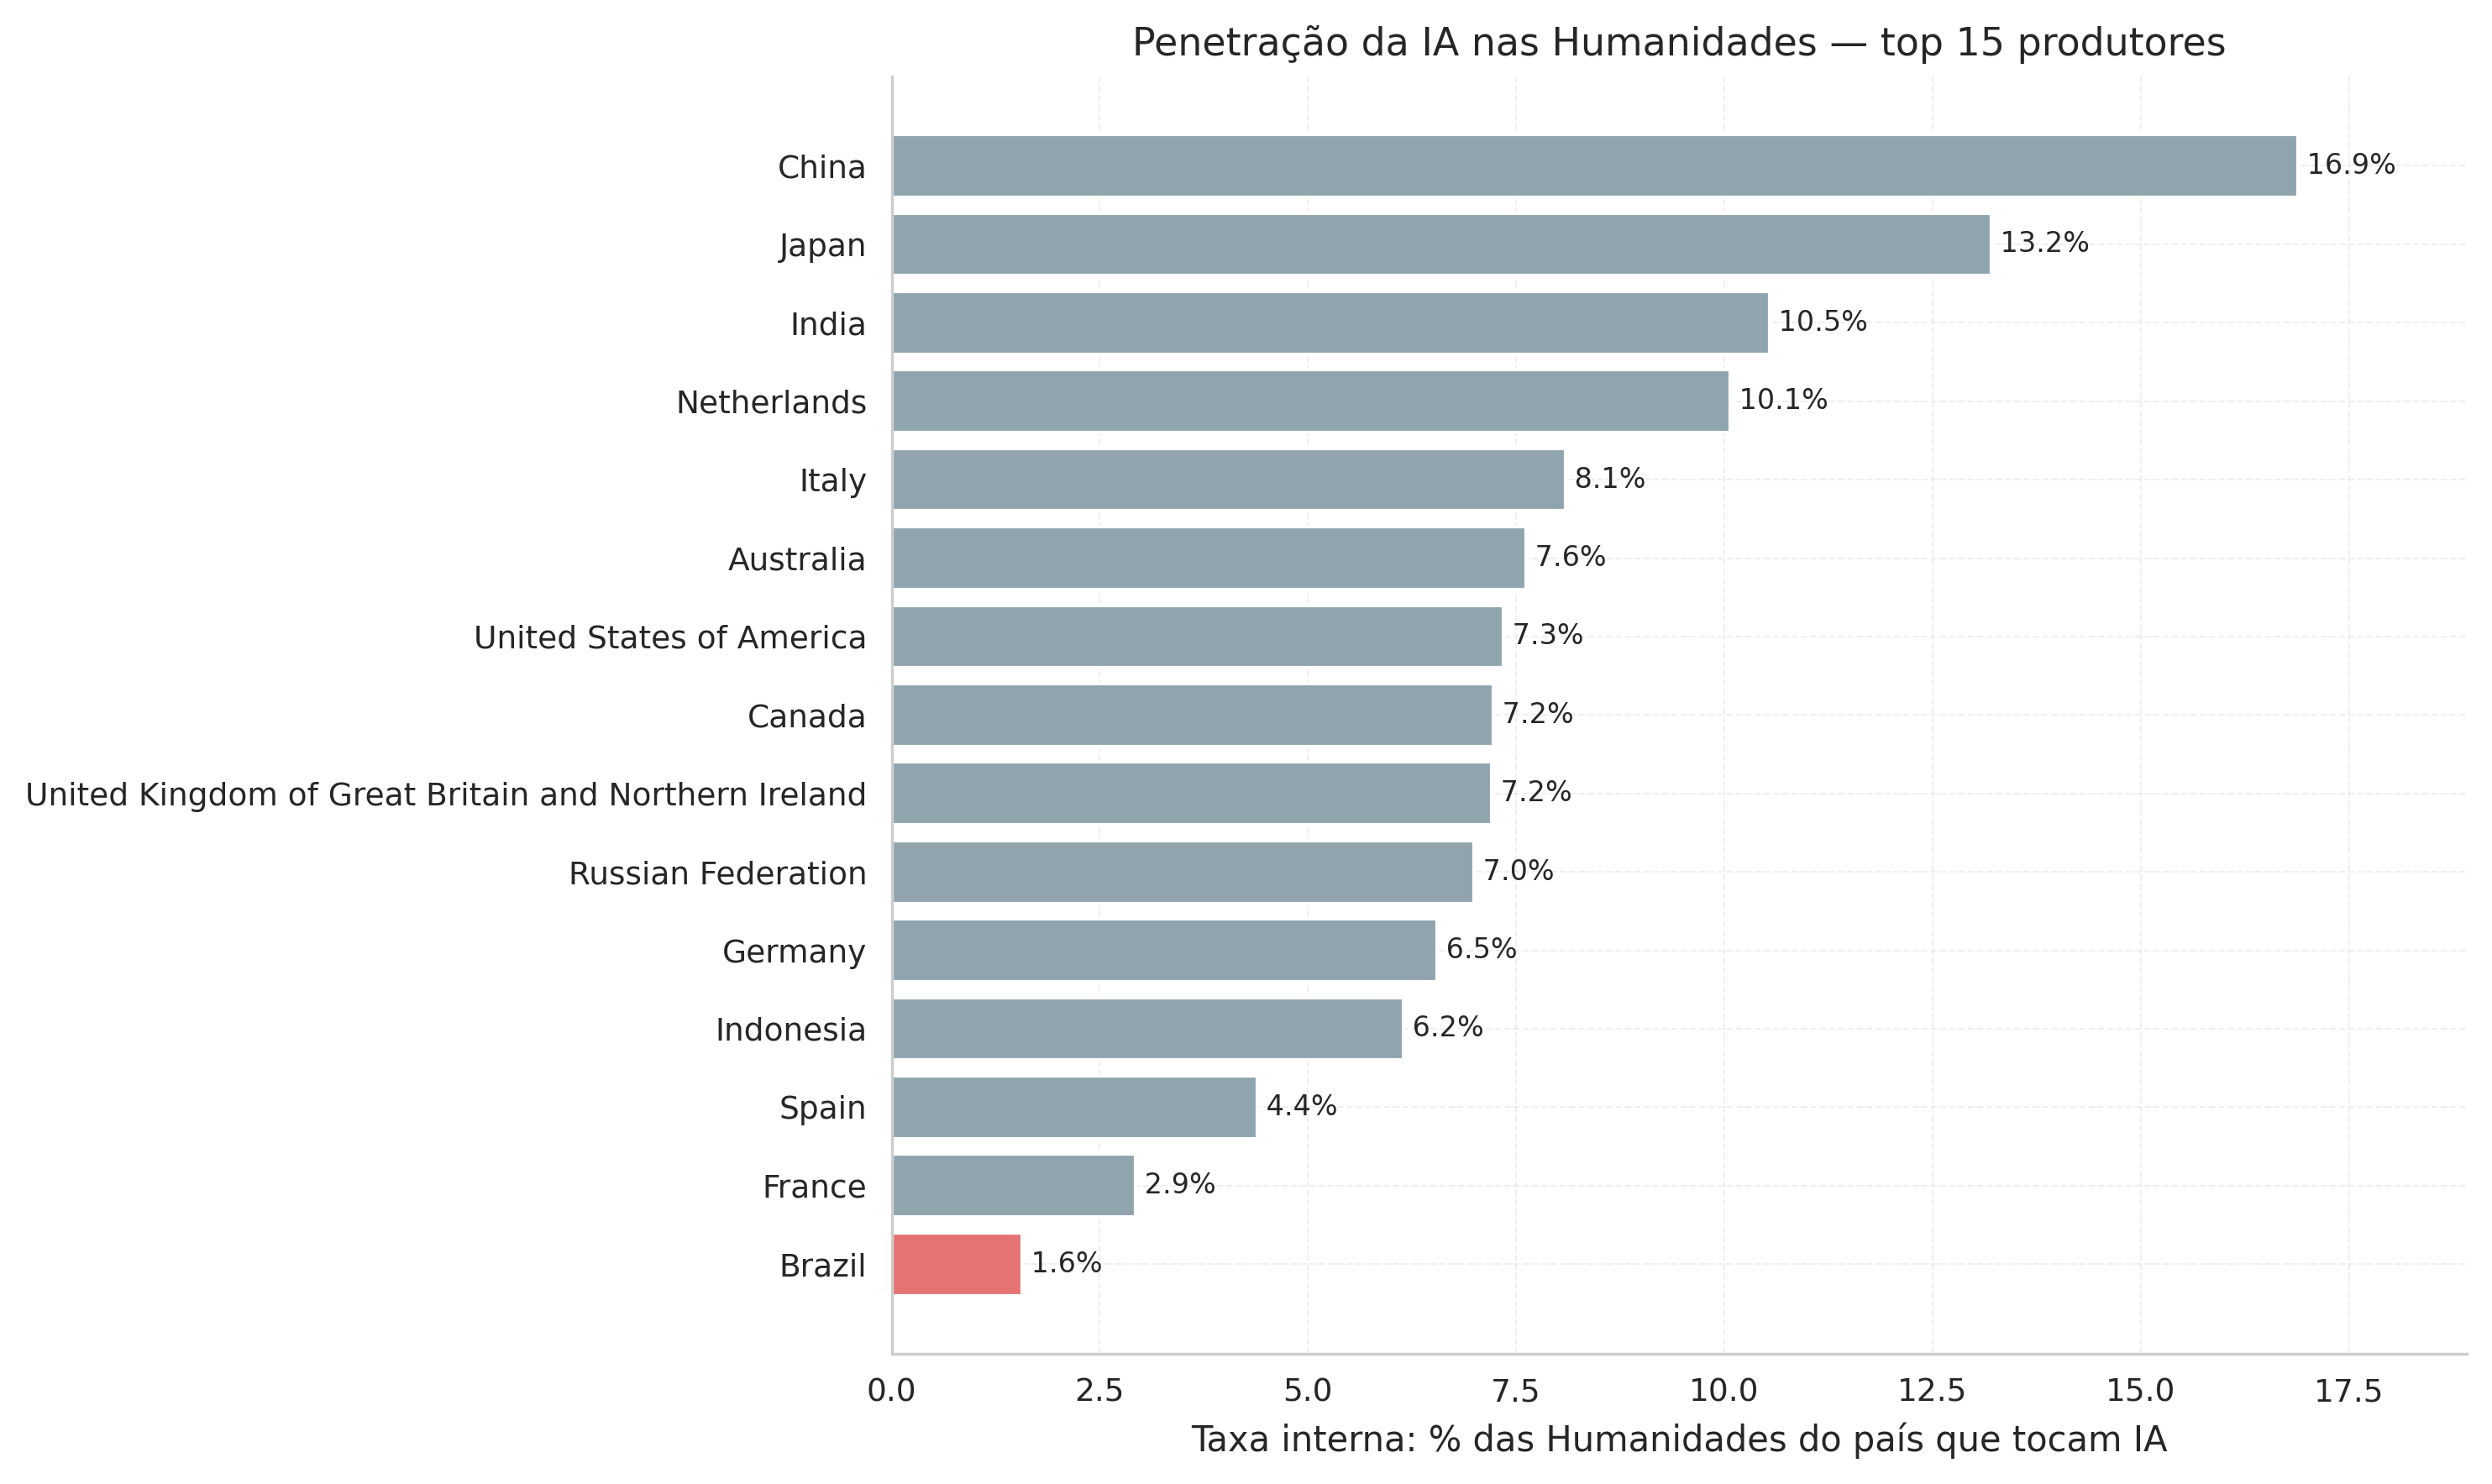
\includegraphics[width=0.95\linewidth]{figuras/openalex_02_taxa_interna_paises.png}
  \caption[Penetração da IA nas Humanidades por país (taxa interna,
  2016--2024)]{Taxa interna --- proporção das publicações de Humanidades de cada
  país que tocam o campo da IA --- entre os quinze maiores produtores,
  2016--2024. Apesar do volume, o Brasil apresenta a menor taxa do grupo
  (1,57\%), contra 16,89\% da China. Fonte: elaboração própria a partir do
  OpenAlex.}
  \label{fig:openalex-taxa}
\end{figure}

A leitura por \emph{taxa interna} --- isto é, a fração das Humanidades de cada
país que dialoga com a IA --- altera radicalmente o quadro
(Figura~\ref{fig:openalex-taxa}). A China lidera a penetração com 16,89\%,
seguida por Japão (13,20\%), Índia (10,54\%) e Países Baixos (10,07\%); os
Estados Unidos, primeiros em volume, exibem penetração intermediária (6,15\%). O
Brasil ocupa o \emph{último} lugar entre os quinze maiores produtores, com apenas
1,57\%. O dado é tanto mais expressivo quando se observa que o Brasil possui o
segundo maior \emph{universo} de Humanidades do conjunto (636.607 obras, atrás
apenas dos Estados Unidos): não se trata, pois, de um país que produz pouco em
Humanidades, mas de um país cuja vasta produção humanística pouco se conecta à
IA. Esse achado replica, em escala internacional, a ``marginalidade'' já
diagnosticada na CAPES (0,67\% das defesas de Humanas tocam a IA) e no
SciELO, conferindo-lhe robustez por triangulação entre fontes independentes.

% ---------------------------------------------------------------------
\begin{figure}[htbp]
  \centering
  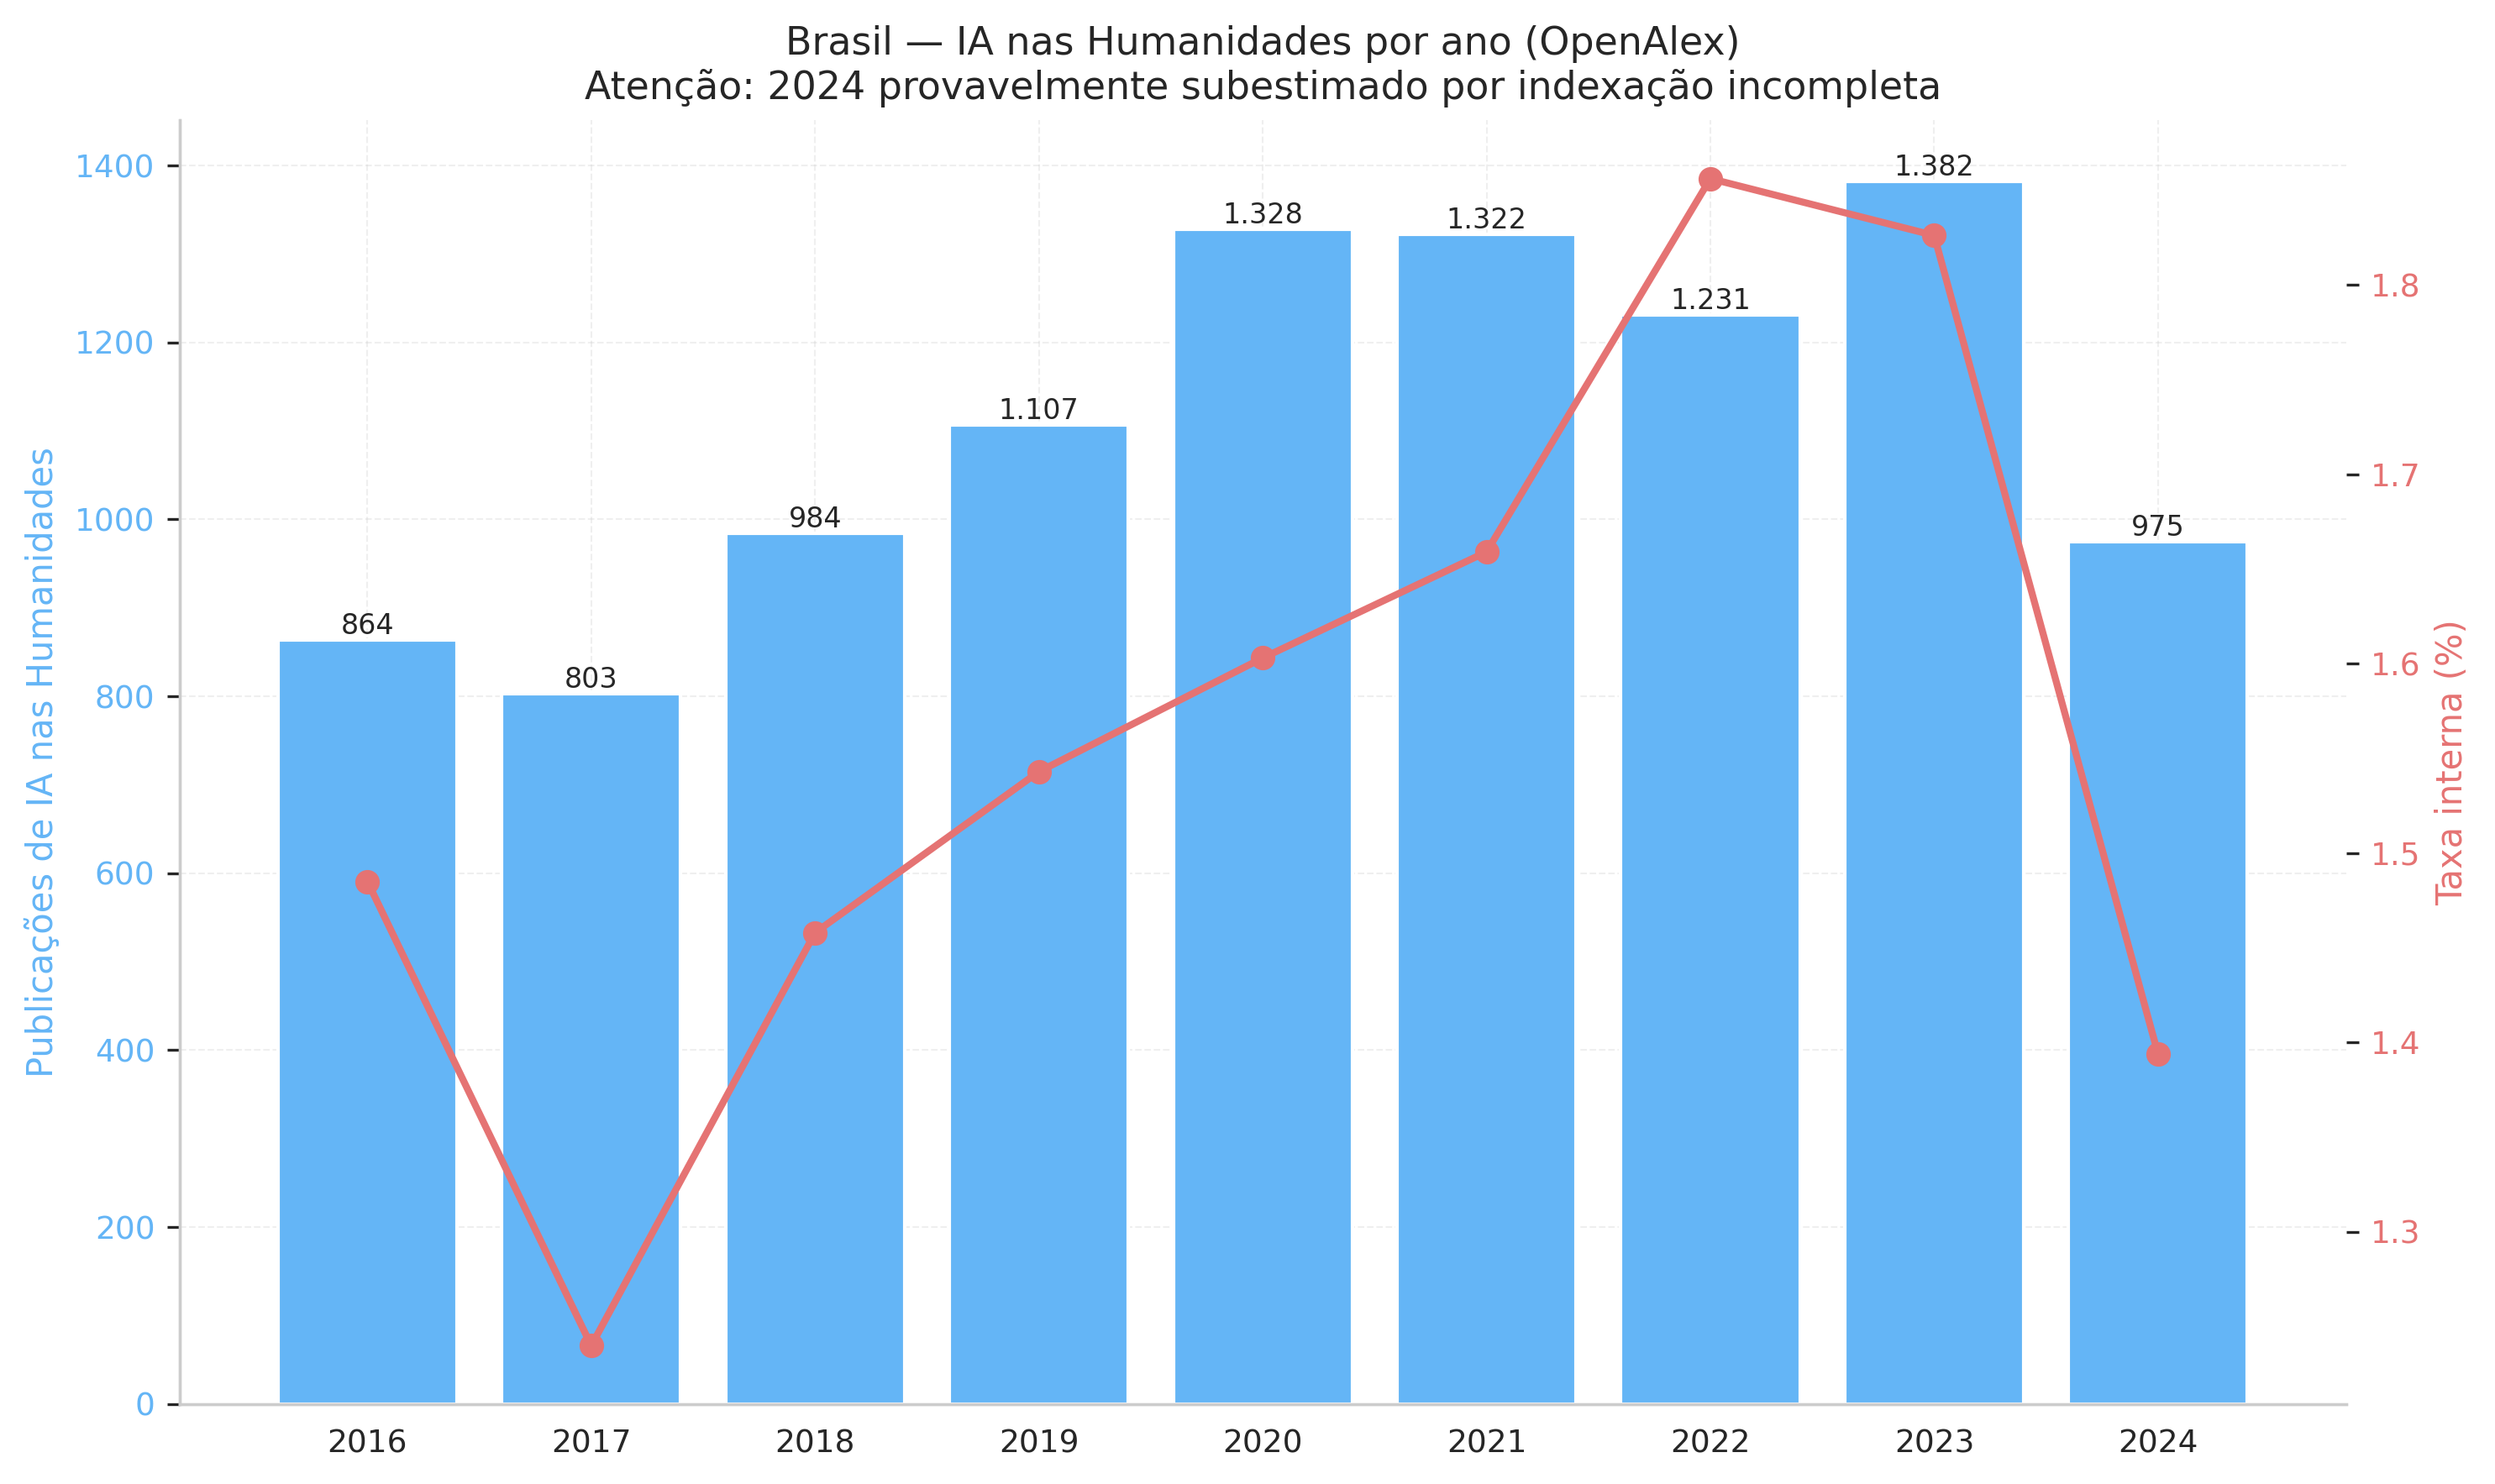
\includegraphics[width=0.95\linewidth]{figuras/openalex_03_brasil_temporal.png}
  \caption[Evolução anual da IA nas Humanidades no Brasil (OpenAlex,
  2016--2024)]{Brasil: volume anual de publicações de IA nas Humanidades
  (barras) e taxa interna (linha), 2016--2024. A retração de 2024 deve-se,
  muito provavelmente, à indexação ainda incompleta do ano no OpenAlex, não a um
  declínio real. Fonte: elaboração própria a partir do OpenAlex.}
  \label{fig:openalex-brasil-temporal}
\end{figure}

A trajetória temporal brasileira (Figura~\ref{fig:openalex-brasil-temporal})
mostra crescimento sustentado entre 2016 (864 obras) e 2023 (1.382 obras),
acompanhado de uma taxa interna que oscila entre 1,2\% e 1,9\%, com pico em 2022
(1,86\%). A aparente queda de 2024 (975 obras) deve ser lida com cautela: o
OpenAlex segue indexando publicações do ano mais recente, de modo que o valor é
quase certamente subestimado --- limitação análoga à observada na própria base
do CSET. O traço marcante não é a flutuação anual, mas a \emph{estabilidade em
patamar baixo} da taxa interna: ainda que o volume cresça, a fração das
Humanidades brasileiras que incorpora a IA permanece estagnada em torno de
1,5\%, o que sugere expansão concentrada em poucos nichos, e não difusão ampla
pelo campo.

% ---------------------------------------------------------------------
\begin{figure}[htbp]
  \centering
  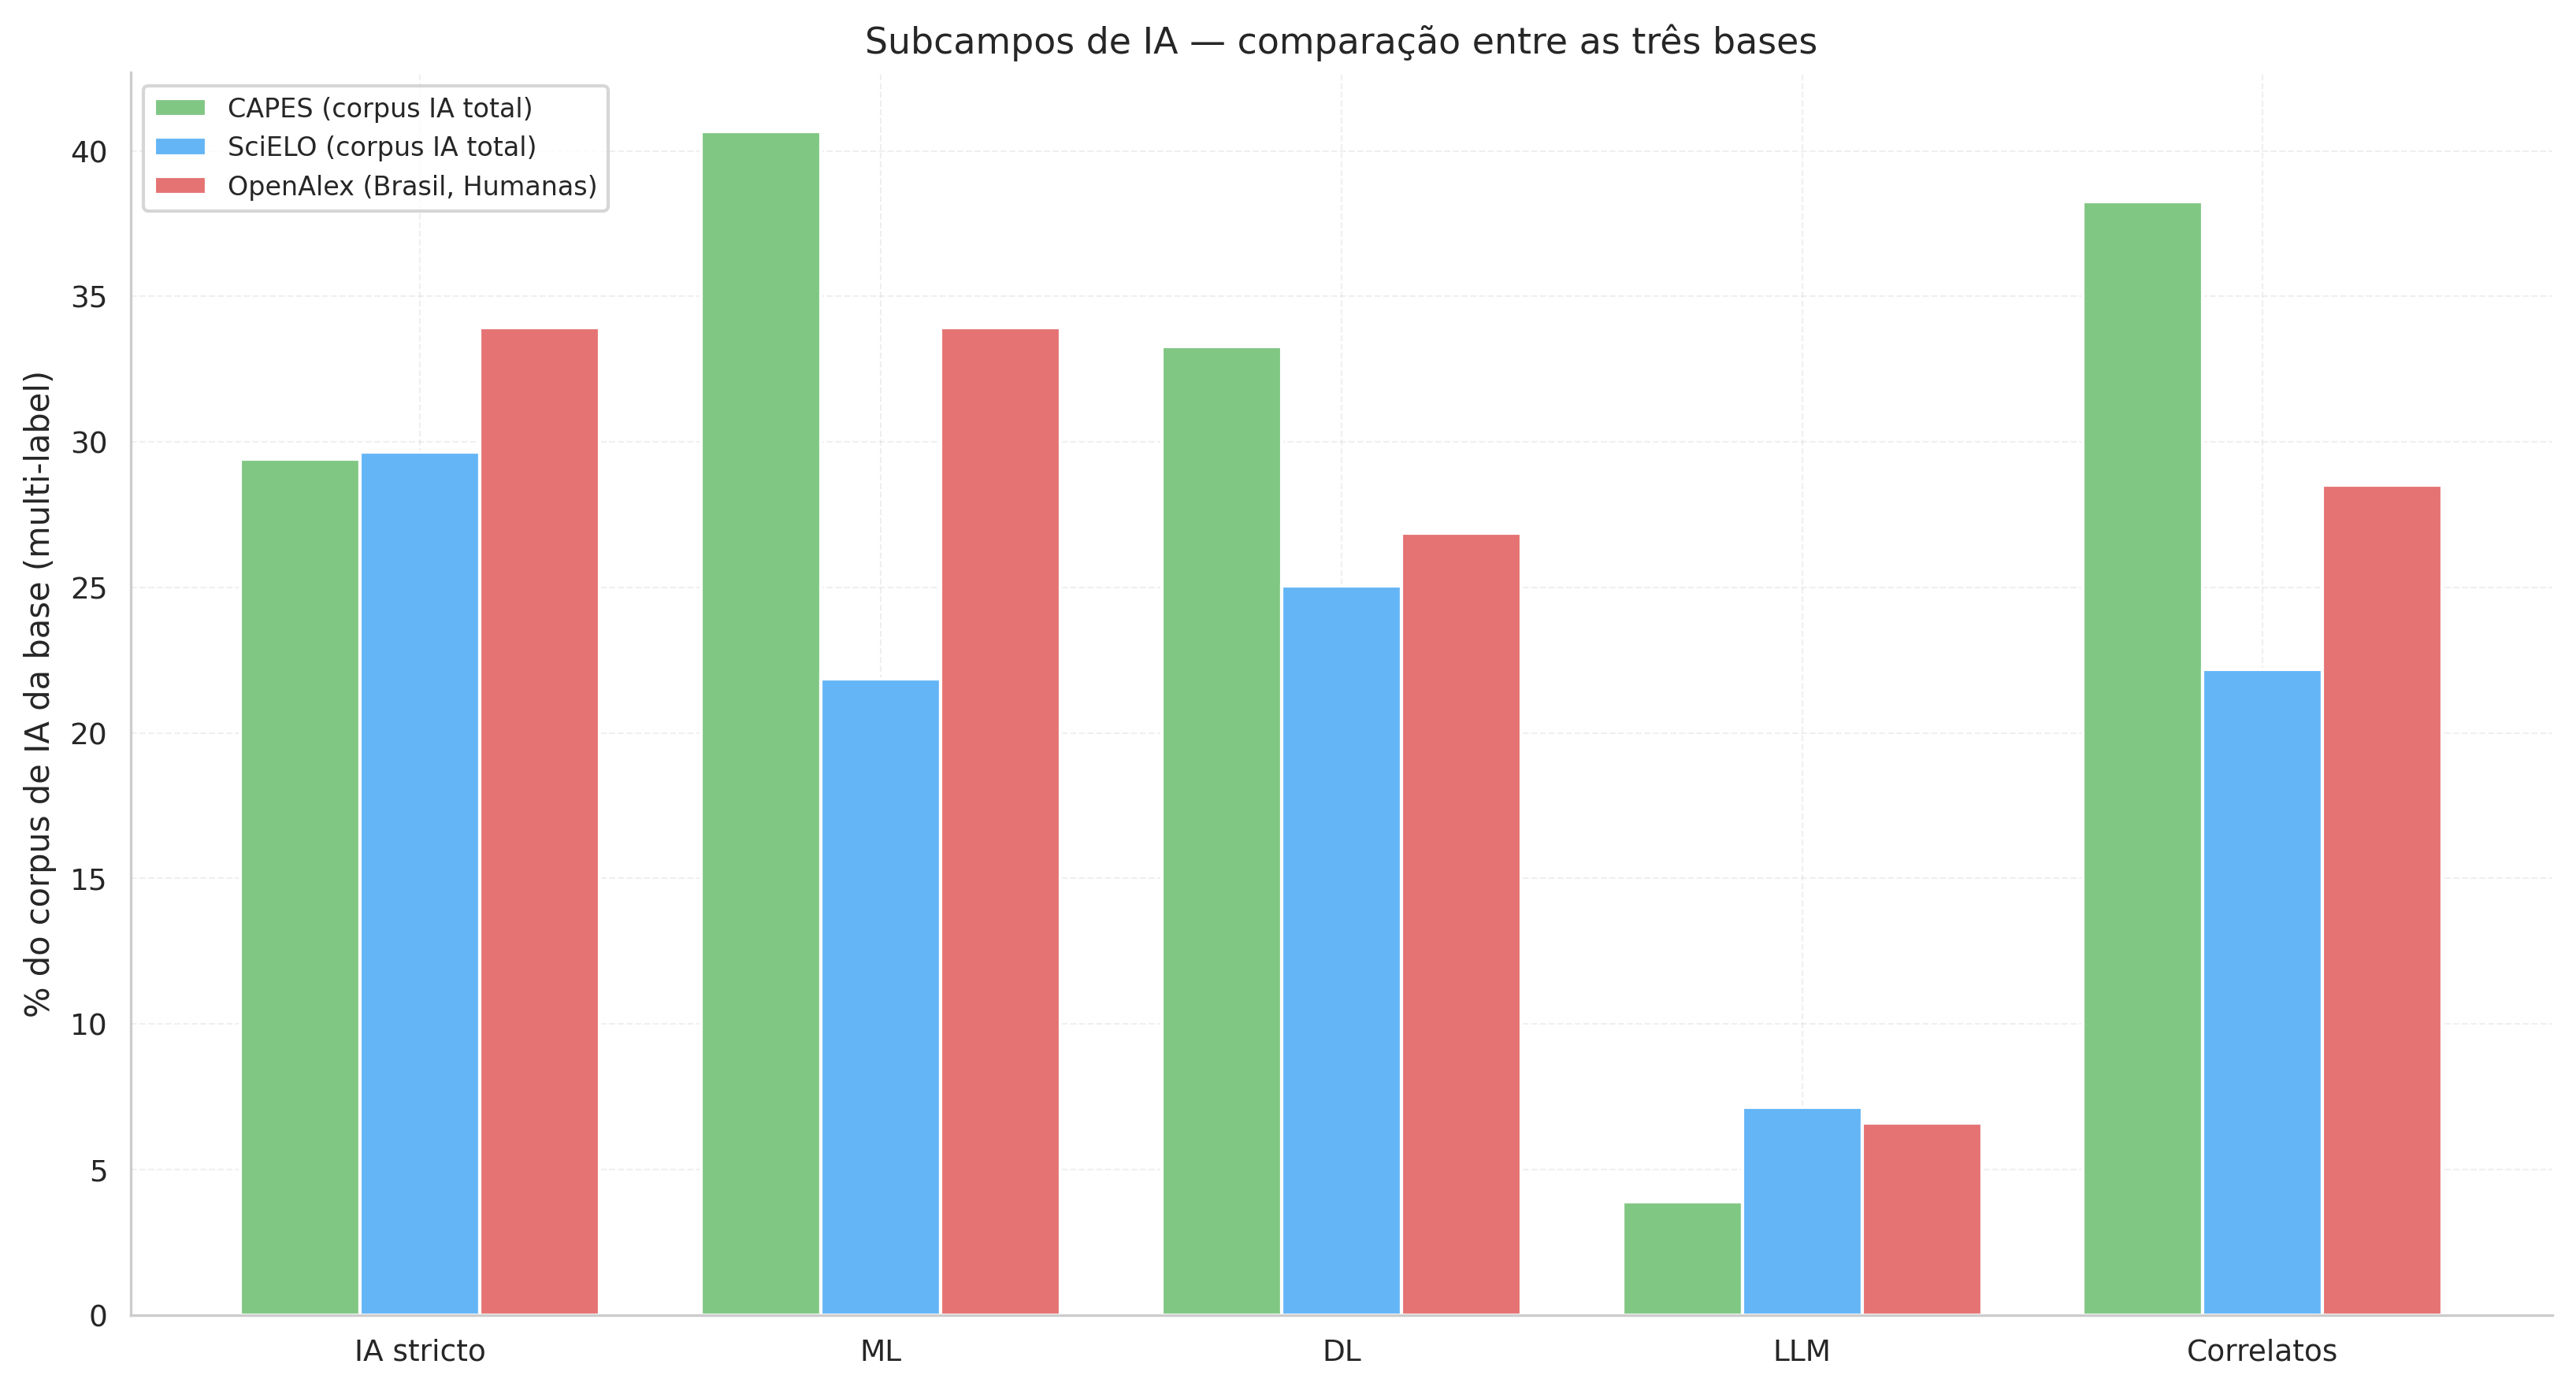
\includegraphics[width=0.95\linewidth]{figuras/openalex_04_subcampos_3bases.png}
  \caption[Distribuição por subcampos de IA: CAPES, SciELO e OpenAlex]{Peso
  relativo dos subcampos de IA (rótulos múltiplos) em cada fonte: CAPES
  e SciELO referem-se ao corpus de IA total da base; OpenAlex, ao recorte de
  Humanidades do Brasil (régua de palavra-chave). Fonte: elaboração própria.}
  \label{fig:openalex-subcampos}
\end{figure}

A Figura~\ref{fig:openalex-subcampos} compara o peso dos subcampos --- IA em
sentido estrito, aprendizado de máquina (ML), aprendizado profundo (DL), modelos
de linguagem e IA generativa (LLM) e tecnologias correlatas --- entre as três
fontes. A comparação deve respeitar uma ressalva de escopo: os percentuais da
CAPES e do SciELO referem-se ao corpus de IA \emph{total} de cada
base, ao passo que os do OpenAlex referem-se ao recorte de Humanidades do Brasil.
Ainda assim, dois padrões se destacam. Primeiro, a hierarquia entre IA estrita e
ML varia conforme a fonte: na CAPES o ML predomina (40,7\% contra
29,4\% de IA estrita), no SciELO a relação se inverte (29,6\% contra 21,9\%), e
no OpenAlex os dois subcampos \emph{empatam} (33,9\% cada). Segundo, os modelos
de linguagem e a IA generativa (LLM) constituem, sistematicamente, o menor
subcampo nas três bases (3,9\% na CAPES, 7,1\% no SciELO e 6,6\% no
OpenAlex) --- indício de que, no período analisado, a virada generativa ainda não
se traduzira em produção acadêmica expressiva nas Humanidades.

% ---------------------------------------------------------------------
\paragraph{Síntese e limitações.} Tomadas em conjunto, as evidências do OpenAlex
internacionalizam o argumento central desta tese: a marginalidade da IA nas
Humanidades brasileiras não decorre de escassez de produção humanística ---
afinal, o país é o segundo maior produtor mundial do conjunto analisado ---, mas
da reduzida permeabilidade desse vasto campo às tecnologias de IA, a menor entre
os grandes produtores. Três limitações devem acompanhar a leitura destes
resultados. \textit{(i)} O OpenAlex privilegia metadados em inglês, o que tende a
subestimar a produção em português (e em chinês), afetando justamente Brasil e
China. \textit{(ii)} Na contagem por país, uma obra é atribuída a cada país de
afiliação de seus autores; os números brasileiros por obra única (bloco
metodológico IV) corrigem essa dupla contagem, mas as comparações internacionais
a mantêm. \textit{(iii)} O ano de 2024 encontra-se subindexado. Nenhuma dessas
limitações, contudo, compromete o achado de fundo, reiterado por três fontes
independentes.
